\documentclass{extarticle}
\usepackage[14pt]{extsizes}
\usepackage{graphicx} % Required for inserting images
\usepackage[T2A]{fontenc}
\usepackage[utf8]{inputenc}
\usepackage[russian]{babel}
\usepackage[center]{titlesec}
\usepackage{indentfirst}
\usepackage[left = 3cm, right = 1cm, top = 2cm, bottom = 2cm]{geometry}
\usepackage{tocloft} %пакет для оформления оглавления
\usepackage[nottoc]{tocbibind} %добавление списка источников в оглавление
\usepackage[titletoc]{appendix} %добавление приложений в оглавление
\usepackage{caption} %заголовки плавающих объектов
\usepackage{csquotes}

\captionsetup[figure]{name=Рисунок}
\bibliographystyle{gost-numeric.bbx}
\usepackage[parentracker=true,
backend=biber,
hyperref=false,
bibencoding=utf8,
style=numeric-comp,
language=auto,
autolang=other,
citestyle=gost-numeric,
defernumbers=true,
bibstyle=gost-numeric,
sorting=ntvy,
]{biblatex}
\addbibresource{library.bib}
\title{DIPLOMA 2}
\author{Евгений Музяев}
\date{May 2024}

\renewcommand{\baselinestretch}{1.25}
\renewcommand{\contentsname}{\normalsize {Содержание}} 
%\renewcaptionname{\appendixname}{Приложение} 
%\renewcommand{\cftchapleader}{\cftdotfill{\cftdotsep}} 

\begin{document}
\begin{titlepage}
%\large 
\begin{spacing}{1}
    \begin{center}
	Министерство науки и высшего образования Российской Федерации\\Санкт-Петербургский Политехнический Университет Петра Великого \\ Физико-механический институт \\ \textbf{Высшая школа фундаментальных физических исследований} 
\end{center}
\begin{flushright}
\begin{tabular}{l}
Работа допущена к защите\\Директор ВШФФИ \vspace{0.3cm} \\
\underline{\hspace{3.5cm}} В. В. Дубов \vspace{0.5cm}\\
«\underline{\hspace{1cm}}»\underline{\hspace{3cm}} 2024 г.
\end{tabular}
\end{flushright}
\vspace{0.3cm}
{ \begin{center}
\vspace{0.3cm}
\MakeUppercase{\textbf{выпускная квалификационная работа \\ магистерская диссертация}}\\
\vspace{0.3cm}

\MakeUppercase{\textbf{Асимметрия Сиверса в полуинклюзивном глубоко неупругом рассеянии лептонов на поперечно поляризованном протоне}}
\\
\vspace{0.5cm}
по направлению подготовки 03.04.02 «Физика»
\\

Профиль $03.04.02\_03$ «Физика ядра и элементарных частиц в фундаментальных и медицинских исследованиях»
\end{center}
}
\vspace{0.3cm}

\begin{flushleft}
	Выполнил \\
	студент гр. 5040302/20301 \hspace{0.3cm} %\hspace{1.9 cm} 
	\hfill  Е.В. Музяев
	\vspace{0.5cm}
	
	
	Научный руководитель\\
	профессор ВШФФИ, д.ф.-м.н.
	\hspace{0.1 cm} \hspace{1.8 cm} 
	\hfill  {Я.А. Бердников}
	\vspace{0.5cm}
	
	Консультант \\
	по нормконтролю \hspace{2.1 cm} \hspace{2 cm} \hfill  {Д.О. Котов}
\end{flushleft}


\begin{center}
	Санкт-Петербург
\end{center}
\begin{center}
    2024
\end{center}
\end{spacing}

\end{titlepage}	



\newpage
\setcounter{page}{2}
\tableofcontents
\newpage
\section*{Введение}\addcontentsline{toc}{section}{Введение}


До сих пор одним из важных вопросов современной физики является исследование спина нуклона. В частности, особый интерес представляет то, как спин нуклона распределяется по его составляющим – кваркам и глюонам. Решение этой задачи позволяет понять устройство материи, а также исследовать эффекты, предсказываемые в рамках Стандартной Модели или найти новые эффекты вне неё. В решении этой проблемы огромную роль играет проведение экспериментов рассеяния лептонов (электронов, позитронов, мюонов) на ядерных мишенях. Несмотря на то, что первые подобные эксперименты были проведены в 50-х годах XX века Робертом Хофштедтером \cite{Hofstadter}, процесс глубоко неупругого рассеяния лептонов на нуклонных и ядерных мишенях до конца не изучен и представляет большой научный интерес.


Изучение процессов глубоко неупругого рассеяния позволяет заглянуть «внутрь» нуклона. Возможно это благодаря размерам частицы-снаряда: лептоны обладают массой и размерами значительно меньшими, чем нуклоны. Например, размер электрона не превышает 0,0001 фемтометра (фм), в то время как размер протона составляет величину 0,74 фм [1].


В 1968 году при проведении экспериментов по глубоко упругому рассеянию (ГНР) на линейном ускорителе электронов SLAC научной группой было установлено [2], что неупругое сечение рассеяния практически не изменяется при изменении переданного импульса $Q^2$, что означает, что структурные функции практически не зависят от $Q^2$. Это явление получило название «скейлинг Бьёркена».


В 1969 году вышла статья Ричарда Фейнмана про партонную структуру частиц. Согласно партонной модели, при больших энергиях нуклоны состоят из безмассовых точечноподобных частиц – партонов. Таким образом, взаимодействие нуклонной материи при высоких энергиях можно представить в виде взаимодействия множества партонов, несущих долю импульса нуклона [3]. При этом предполагается, что импульс партонов коллинеарен импульсу нуклона. Распределение кварков по импульсу внутри нуклона можно описать партонной функцией распределения (ПФР).


В 1986 г. в эксперименте по рассеянию поляризованных µ-мезонов на поляризованных протонах в Европейской-мюонной коллаборации (EMC) был получен удивительный результат – суммарный спин валентных кварков даёт вклад, равный лишь 33\% от спина нуклона [4]. Данная проблема получила название «спиновый кризис». Для исследования этой проблемы были проведены эксперименты HERMES (HERA Spin MESurement) [5] и COMPASS (COmmon Muon Proton Apparatus for Structure and Spectroscopy) [6], в которых рассматривались явления полуинклюзивного (с рождением и регистрацией выделенного мезона) глубоко неупругого рассеяния (ПГНР) лептонов на поперечно поляризованном протоне. В результате этих экспериментов была обнаружена азимутальная асимметрия образовавшихся мезонов.


Азимутальная асимметрия – отношение разности сечений рассеяния образовавшихся адронов влево и вправо на одинаковые углы в одной плоскости к сумме тех же сечений [7]:
\begin{equation}
    A_N =\frac{d\sigma^\uparrow -d\sigma^\downarrow }{d\sigma^\uparrow +d\sigma^\downarrow },
\end{equation} 
где $A_N$ - азимутальная асимметрия, $d\sigma^\uparrow$  – сечение образовавшихся адронов в левой плоскости, $d\sigma^\downarrow$  – в правой плоскости.


 В эксперименте по рассеянию пучка поляризованных протонов на поляризованной водородной мишени, проведённых коллаборацией E704 в лаборатории Ферми, было обнаружено, что азимутальная асимметрия образовавшихся $\pi^0$-мезонов растёт с увеличением поперечного импульса и переменной Фейнмана $x_F$, что не нашло объяснений в рамках коллинеарной пертурбативной квантовой хромодинамики (КХД) [8]. Для объяснения этого эффекта были предложены партонные функции распределения, и функции фрагментации (ФФ), зависящие от величины поперечного импульса кварков.

 
 Измерение неколлинеарных партонных функций распределения кварков и глюонов важно для исследования внутренней структуры нуклона. Существует несколько способов измерения: исследование процессов Дрелл-Яна, образования прямых фотонов и полуинклюзивного глубоко неупругого рассеяния. 

\textit{Целью работы} является моделирование расчёта односпиновой азимутальной асимметрии Сиверса образовавшихся адронов в глубоко неупругом рассеянии лептонов на нуклоне - мишени с использованием Монте-Карло генератора событий PYTHIA8 и плагина Stringspinner, учитывающего эффекты поляризации частиц. 

В Главе 1 представлено введение в кинематику глубоко неупругого рассеяния, в главе 2 рассмотрены основы партонной модели и поляризация кварков, в 3-ей главе рассмотрена фрагментация кварков,  в 4-ей главе -- азимутальные асимметрии в процессах глубоко неупругого рассеяния на поперечно поляризованной мишени, в 5-ой главе представлено моделирование процессов ГНР на поляризованной мишени в Монте-Карло генераторе PYTHIA8, в 6-ой главе произведён расчёт асимметрий Сиверса в процессах рассеяния неполяризованных лептонов на поперечно поляризованной мишени и представлены результаты этого расчёта.

\newpage
\section{Глубоко неупругое рассеяние}
Глубоко неупругое рассеяние – процесс неупругого взаимодействия леп-тона (электрона, мюона, нейтрино) и сильно взаимодействующей частицы – нуклона (протон, нейтрон), протекающего при энергетическом масштабе сильно большем, чем сумма масс покоя участников взаимодействия.
\subsection{Кинематика глубоко неупругого рассеяния}
Рассмотрим глубоко-неупругое рассеяние электрона на протоне в приближении однофотонного обмена (дальнейшие рассуждения по этой теме справедливы и для других частиц – мюонов и нейтронов). При таком приближении предполагается, что лептон с нуклоном обмениваются виртуальным фотоном. Обозначим импульс протона через $P$, начальный и конечный импульс электрона – через $k$ и $k'$. Тогда можно вычислить вектор импульса, переданный виртуальным фотоном адронной системе как $q=k-k'$. Вектор \textit{q} неинвариантен (его величина зависит от выбора системы координат), поэтому принято пользоваться инвариантным квадратом импульса $q^2=-Q^2$.

Если величина переданного импульса $Q^2$ велика, то кварк «излучается» из нуклона так, что мягкие процессы не смогут сбалансировать реакцию. В таком случае лептон передаст импульс не всему нуклону как целому, а определённому кварку. Но несмотря на это, мягкие процессы не исчезнут – будут образовываться глюоны и кварк-антикварковые пары, и цветной кварк преобразуется в бесцветные адронные струи. Такой процесс называется фрагментацией, о котором речь пойдёт позже.

Упрощённая диаграмма процесса глубоко неупругого рассеяния на кварковом уровне представлена на Рисунке \ref{fig:DIS}.
\newpage

\begin{figure}[h!]
    \centering
    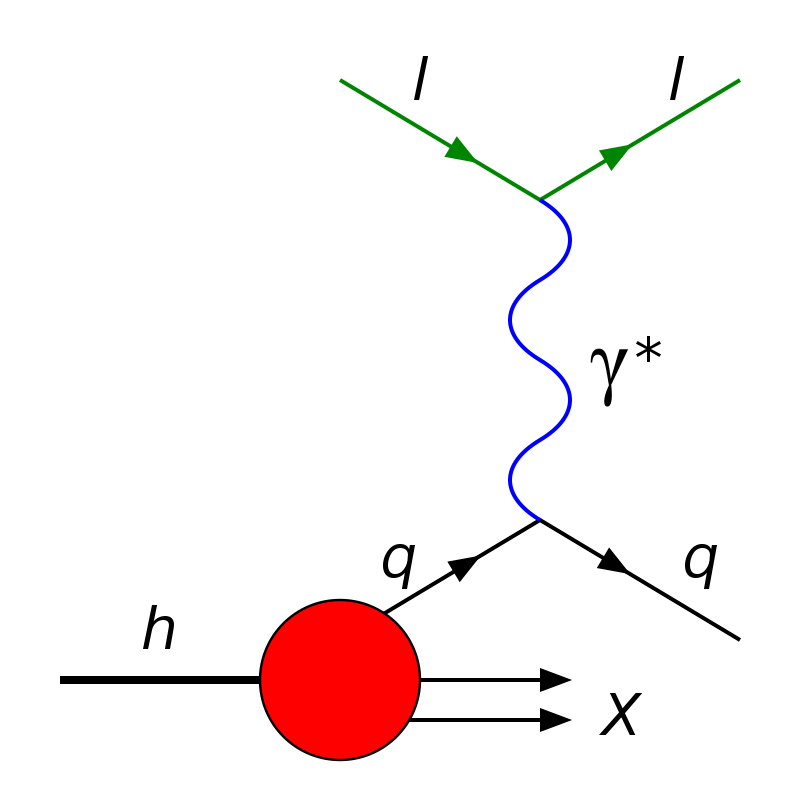
\includegraphics[width = 0.7\linewidth]{DIS.png}
    \caption{Упрощённая диаграмма глубоко неупругого рассеяния в приближении однофотонного обмена}
    \label{fig:DIS}
\end{figure}

Здесь налетающий лептон $l$ взаимодействует с кварком $q$ нуклона $h$, обмениваясь виртуальным фотоном $\gamma*$. Символом $X$ обозначены "остатки"\  адрона - частицы, не участвующие в реакции.

Рассмотрим глубоко неупругое рассеяние электрона на протоне в системе центра масс. В этой системе электрон и протон будут лететь навстречу друг другу. Энергия в системе центра масс велика, поэтому массу протона можно игнорировать, следовательно, импульс протона будет подобен импульсу безмассовой частицы (фотона). Импульс составляющих протон кварков будет коллинеарен импульсу протона (практика показывает, что кварки обладают ненулевым поперечным импульсом). Таким образом, кварки будут нести часть импульса нуклона. Для описания этого вводится безразмерная переменная Бьёркена $x_{Bj}$, которая определяется как доля импульса нуклона, которую несёт кварк:
\begin{equation}
    x_{Bj}= \frac{Q^2}{2Pq},
\end{equation}
где \textit{P} -- импульс нуклона, \textit{q} -- переданный импульс. 
Таким образом, импульс \textit{p} кварка адрона \textit{h}, обладающего импульсом $P$ можно выразить как
\begin{equation}
    p=x_{Bj}P.
\end{equation}
По определению величина переменной Бьёркена положительна и не превышает единицы: 
\begin{equation}
    0 < x_{Bj} \leq 1.
\end{equation}
Переменная Бьёркена равняется единице в случае упругого рассеяния, если меньше единицы - то неупругое.

Введём кинематическую переменную $y$, выражающую относительную потерю энергии налетающей частицы-лептона:
\begin{equation}
    y = \frac{P \cdot q}{P \cdot k},
\end{equation}
где $q$ - импульс виртуального фотона, $k$ - начальный импульс лептона. По определению, переменная $y$ не может превышать единицы.

Потерю энергии налетающей частицы в системе центра масс можно выразить как 
\begin{equation}
    \nu = \frac{P \cdot q}{M},
\end{equation}
где $M^2 = P^2$ -- масса нуклона-мишени. Переменную Бьёркена можно выразить через эту величину:
\begin{equation}
    x_{Bj} = \frac{Q^2}{2M\nu}
\end{equation}


\subsection{Сечение глубоко неупругого рассеяния}

Физика элементарных частиц рассматривает процессы, происходящие на квантовомеханических масштабах. Изучение таких процессов требует вероятностного подхода описания событий. Одним из таких способов изучения взаимодействия элементарных частиц является нахождение дифференциального и интегрального сечений рассеяния. По величине сечения рассеяния можно определить вероятность того или иного процесса - распада, образования новых частиц и т.д. Чем больше величина сечения рассеяния, тем выше вероятность этого процесса.

Дифференциальное сечение рассеяния в лабораторной системе определяется следующим образом:
\begin{equation}
    \frac{d\sigma}{d\Omega}(\theta) = \frac{\frac{dN}{d\Omega}(\theta)}{I \cdot n},
\end{equation}
где $\theta$ -- угол рассеяния, $I$ -- поток налетающих частиц, $n$ -- число частиц мишени, $\Omega$ -- телесный угол, $\frac{dN}{d\Omega}$ -- число частиц, вылетевших в единичном элементе телесного угла $\Omega$ за единицу времени.

Полное (эффективное) сечение рассеяния можно получить, проинтегрировав по углу:
\begin{equation}
    \sigma = \int \frac{d\sigma}{d\Omega}d\Omega. 
\end{equation}
Эффективное сечение рассеяния характеризует вероятность взаимодействия налетающей частицы с частицей-мишенью. Полное эффективное сечение рассеяния складывается из сечений упругого рассеяния и неупругого:
\begin{equation}
    \sigma = \sigma_{el} + \sigma_{inel},
\end{equation}
где $\sigma_{el}$ -- сечение упругого рассеяния, $\sigma_{inel}$ -- сечение неупругого рассеяния. 

Дифференциальное сечение электрона на ядре с числом протонов $Z$ выражается как 
\begin{equation}
    \frac{d\sigma}{d\Omega} = ( \frac{d\sigma}{d\Omega})_{Mott} |F(q)|^2 ,
\end{equation}
где $\Omega$ - телесный угол, $F(q)$ -- форм-фактор, $q = k-k'$ -- переданный импульс. Выражение в скобках означает сечение Мотта -- рассеяние электрона на точечной частице:
\begin{equation}
    (\frac{d\sigma}{d\Omega})_{Mott} = \frac{(Z\alpha)^2 E^2}{4k^4 \sin^4 (\theta/2)} (1- \frac{k^2}{E^2} \sin^2(\theta/2)),
\end{equation}
где $Z$ - электрический заряд частицы, $\theta$ - угол рассеяния, $E$ - энергия рассеянной частицы. Таким образом, форм-фактор $F(q)$ возникает, когда частица-мишень является составной. Форм-фактор зависит от распределения составляющих ядро частиц и равен Фурье-образу плотности распределения электрического заряда:
\begin{equation}
    F(q) = \int \rho(r) \exp^{\frac{i}{\hbar}qr}dr,
\end{equation}
где $\rho(r)$ -- плотность распределения, $r$ -- радиус-вектор из центра ядра, $\hbar$ -- приведённая постоянная Планка.

В работе \cite{Breidenbach} было показано, что при увеличении энергии центра масс реакции происходит уменьшение упругой части рассеяния. На графике \ref{fig:Mott} показано отношение сечения рассеяния электрона на протоне к сечению Мотта при энергиях центра масс 2, 3, 3,5 ГэВ. Отдельной линией выделено сечение упругого рассеяния, которое падает с увеличением квадрата переданного импульса. Это говорит о том, что протон составная частица. 
\begin{figure}[ht]
    \centering
    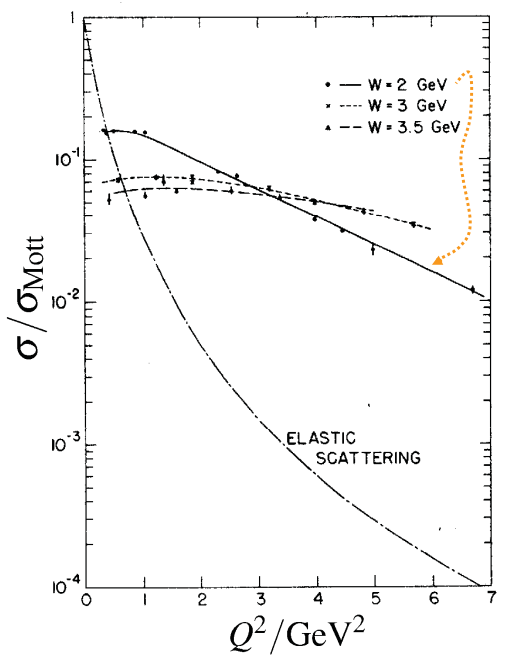
\includegraphics[width = 0.6\linewidth]{Mott.png}
    \caption{Отношение дифференциального сечения рассеяния по углу и энергии к сечению Мотта \cite{Breidenbach}.}
    \label{fig:Mott}
\end{figure}

Однако поведение неупругого рассеяния показывает другие результаты - его величина слабо зависит от $q^2$. Таким образом, сечение неупругого рассеяния приблизительно обладает единичным форм-фактором, что говорит о том, что электрон рассеивается на точечной частице, которая является составляющей нуклона.



\newpage
\section{Партонная модель}
Партонная модель описывает процессы, которые происходят внутри ядер и адронов. Основой партонной модели служит утверждение, что при энергиях сильно больших, чем инвариантная масса нуклона, взаимодействие между элементарными частицами можно представить через взаимодействие множества партонов. Таким образом, партон -- точечноподобная безмассовая частица, несущая долю импульса адрона. Как правило, партоны отождествляют с кварками и глюонами. 
Таким образом, нуклон при $Q^2 >> M^2$ можно представить в виде "шубы"\ из множества кварков и глюонов, которые в том числе взаимодействуют между собой.
\subsection{Скейлинг Бьёркена и структурные функции}

В 1968 году Дж. Бьёркен предположил, что в пределе $Q^2$ на бесконечности, структурные функции должны зависеть только от переменной Бьёркена $x_{Bj}$.  

\subsection{Партонные функции распределения}
Поведение кварков в нуклоне можно описать партонной функцией распределения $f(x_{Bj},Q^2)$ – плотности вероятности обнаружить в адроне партон, обладающего долей импульса $x_{Bj}$ при энергетическом масштабе взаимодействия $Q^2$. Вычислить ПФР можно только исходя из экспериментальных данных. Партонные функции распределения разделяют на коллинеарные (импульс партона сонаправлен с импульсом адрона) и неколлинеарные (партоны имеют ненулевую составляющую поперечного импульса).
\subsubsection{Коллинеарные партонные функции}
Начнём рассмотрение партонной модели с коллинеарных функций распределения. 
\newpage
\subsection{Поляризация частиц}

 В физике достаточно изучена электромагнитная поляризация волн – направленное в определённой плоскости колебание векторов \textbf{E} и \textbf{H}. Поляризация частиц имеет другую природу и выражается в преимущественной ориентации спина частицы вдоль выбранного направления по отношению к её импульсу. Поляризацию частиц разделяют на поперечную (спин частицы перпедикулярен её импульсу) и продольную (спин частицы коллинеарен импульсу). 
 Охарактеризовать поляризацию частицы можно через спиральность:
 \begin{equation}
     h = \frac{\textbf{S} \cdot \textbf{P}}{|S|\cdot |P|}
 \end{equation}
%h=(S⃗⋅P⃗)/(|S⃗|⋅|P⃗|) ,
где \textbf{S} – вектор спина частицы, \textbf{P} – вектор импульса. Если спиральность частицы по модулю равняется единице, то она поляризована продольно, если спиральность равна нулю, то поперечно. 


 Величина спина нуклона общеизвестна – 1/2, но до сих пор неизвестно распределение спина нуклона по его составляющим (конституэнтам), или, что аналогично, из чего складывается этот спин. До публикации результатов коллаборации EMC [4] считалось, что спин нуклона полностью складывается из спинов валентных кварков (те кварки, которые определяют квантовые числа адронов). Данный эксперимент показал, что валентные кварки дают вклад, равный лишь трети от суммарного спина. На данный момент достоверно известно, что спин в том числе распределяется по валентным кваркам, морским кваркам, глюонам и орбитальным моментам этих частиц. На рисунке 4 схематично представлена картина возможного распределения спина нуклона по его составляющим.
 Однако, как оказалось, недостающие 70\% спина зависят не только лишь от орбитального момента кварков и глюонов \cite{Hagler}, и существует ненулевая корреляция между направлением спина партонов и их импульсов в нуклоне. 

\begin{figure}[ht]
    \centering
    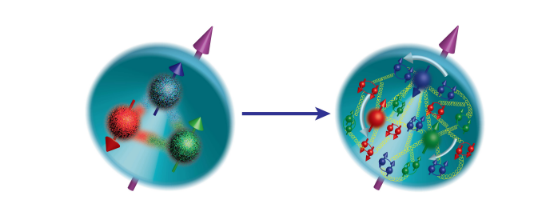
\includegraphics[width = 0.9\linewidth]{nucleo.png}
    \caption{Схематичное изображение эволюции представлений о внутренней структуре спина нуклона: слева – устаревшее представление, справа – современное представление}
    \label{fig:nucleo}
\end{figure}
 

 В лидирующем порядке квантовой хромодинамики поляризованный нуклон можно описать тремя ПФР кварков – функцией $f_1^q$, которая показывает распределение неполяризованных кварков в неполяризованном нуклоне, спиральностью $g_1^q$, которая описывает кварки с продольной поляризацией в продольно поляризованном нуклоне, и «трансвёрсити» (поперечная поляризация) $h_1^q$, которая описывает распределение поперечно поляризованных кварков в поперечно поляризованном нуклоне [13]. Среди этих трех неколлинеарных партонных функций распределения «трансвёрсити» является менее изученной и наиболее труднодоступной из-за её киральной нечетной природы. Киральная нечётность означает, что при зеркальном отображении системы относительно оси координат симметрия системы не будет сохраняться.
Для измерения функции «трансвёрсити» необходимо изучение процесса, в котором участвуют две кирально-нечётные функции. Такую возможность даёт изучение азимутальных асимметрий адронов в полуинклюзивном глубоко неупругом рассеянии на поперечно поляризованной мишени.

\newpage

\section{Фрагментация и адронизация кварков}
Результатом процесса глубоко неупругого рассеяния является образование большого числа частиц в результате сильного взаимодействия кварков. Процесс возникновения бесцветных адронов (частиц-участников ядерного взаимодействия) из цветных кварков называется фрагментацией.
\subsection{Модель адронизации Лунда}
Рассмотрим простейшую Лундовскую модель адронизации (йо-йо модель) [10]. Процесс адронизации удобно представить на следующей схеме: 
\begin{figure}[h]
    \centering
    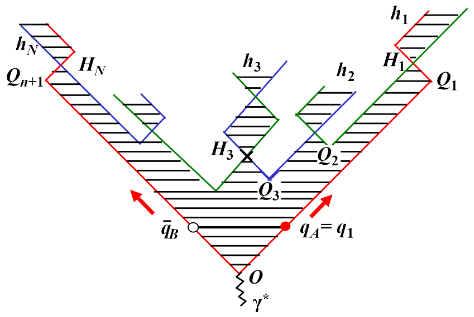
\includegraphics[width = 0.7\linewidth]{fragmentation.png}
    \caption{Схематичное изображение процесса адронизации}
    \label{fig:hadronization}
\end{figure} 
\\
Здесь \textbf{O} – точка взаимодействия партона $q_A$ с виртуальным фотоном $\gamma*$, с которой начинается процесс адронизации; $\textbf{Q}_i$ – точки(узлы) разрыва струны, где $i = 1, 2, \dots, n$; \textbf{H} -- точки образования адронов $h_i$, где $i = 1, 2, \dots, n$.

Процесс начинается со взаимодействия виртуального фотона $\gamma*$, испущенного налетающим лептоном, с партоном мишени \textit{q} (здесь и далее предполагается, что взаимодействуют кварки, но последующие рассуждения справедливы и для глюонов). Виртуальный фотон передаёт кварку $A$ импульс, вследствие чего кварк $q_A$ начинает отдаляться от кварка $B$ оставшегося «раненого» нуклона. 

\subsection{Модель 3P0}
\newpage
\section{Азимутальные асимметрии}

\subsection{Асимметрия Коллинза}
\subsection{Асимметрия Сиверса}
\newpage
\section{Эксперимент HERMES}
\subsection{Асимметрии образовавшихся пионов}
\subsection{Асимметрии образовавшихся каонов}
\newpage
\section{Моделирование процессов в PYTHIA}
\subsection{Поляризация в PYTHIA}
\newpage


\printbibliography

\end{document}
